% TODO: replace this image with our own renders
\begin{figure}[H]
	\centering
	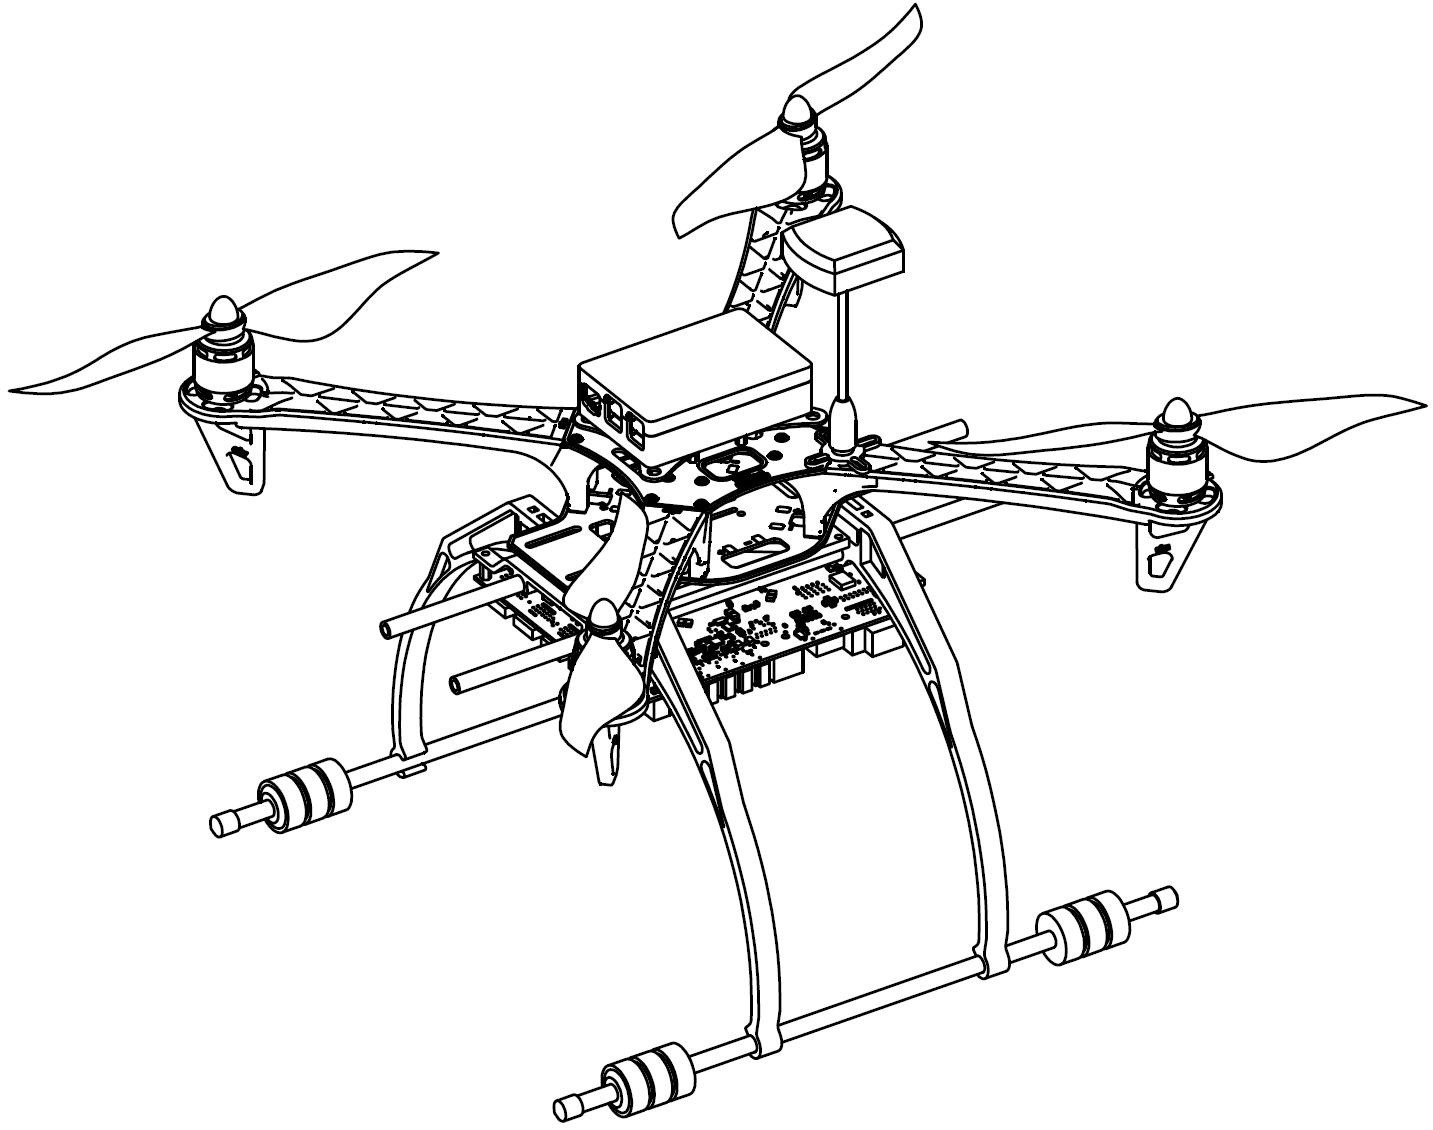
\includegraphics[width=0.85\textwidth]{img/testrigcad1.png}
	\caption[Team 109 Testing Rig Prototype]{Team 109 Testing Rig Prototype using RPAS Generously Provided by Yiyi Yan and UBC \textit{Unmanned Aerial Systems}}
	\label{fig:testrigcad1}
\end{figure}

A remote-piloted aerial system (RPAS) or sometimes referred to as ``drone" and ``multirotor" consists of serveral subsystems: airframe, mechanical structures, propulsion, battery, sensors, and flight computer. This section will explore these subsystems in more detail. Figure~\ref{fig:testrigcad1} is a render of the completed mutlirotor with the computing platform payload attached.

\subsubsection{Mechanical}\label{section:drone-mech}
The mechanical subsystem of the multirotor is comprised of the frame that holds all the propulsion system, on-board computer and sensors, and the payload together.

\paragraph{Frame Configuration}

\begin{figure}[b]
	\centering
	\begin{subfigure}[b]{0.3\textwidth}
		\centering
		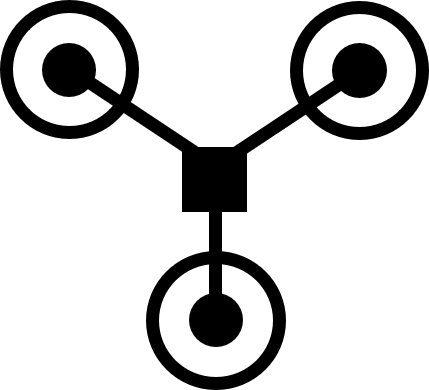
\includegraphics[scale=0.4]{img/drone_yconfig}
		\caption{Tricopter Y-Configuration}
		\label{fig:tricopter-y}
	\end{subfigure}
	~
	\begin{subfigure}[b]{0.3\textwidth}
		\centering
		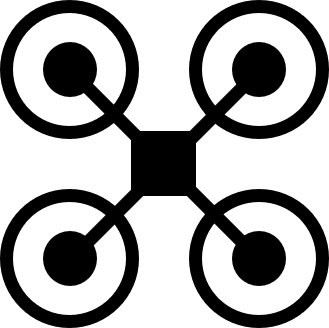
\includegraphics[scale=0.4]{img/drone_xconfig}
		\caption{Quadcopter X-Configuration}
		\label{fig:quadcopter-x}
	\end{subfigure}
	~
	\begin{subfigure}[b]{0.3\textwidth}
		\centering
		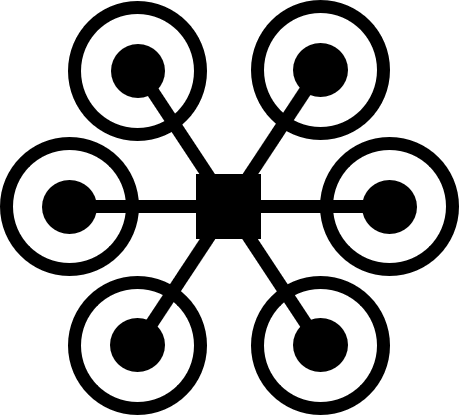
\includegraphics[scale=0.4]{img/drone_hexconfig}
		\caption{Hexcopter X-Configuration}
		\label{fig:hexcopter-x}
	\end{subfigure}
	
	\caption{Multirotor RPAS Configurations}
	\label{fig:rpas-config}
\end{figure}

\begin{figure}[h]
	\centering
	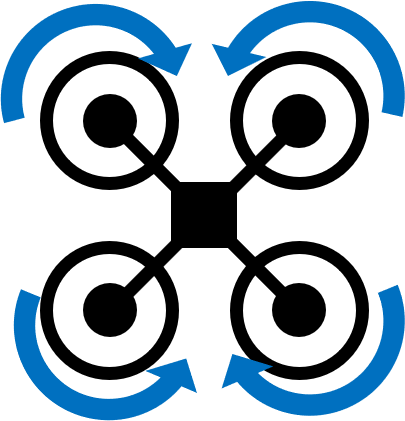
\includegraphics[scale=0.4]{img/drone_xconfigt}
	\caption{Quadcopter X-configuration}
	\label{fig:quadcopter-x-t}
\end{figure}

\begin{figure}[h]
	\centering
	\begin{subfigure}[b]{0.3\textwidth}
		\centering
		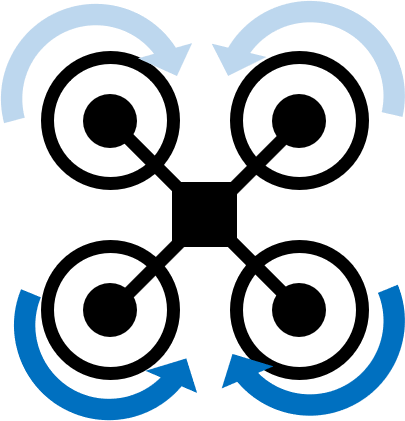
\includegraphics[scale=0.4]{img/drone_x_pitch}
		\caption{Pitch forward}
		\label{fig:x-pitch}
	\end{subfigure}
	~
	\begin{subfigure}[b]{0.3\textwidth}
		\centering
		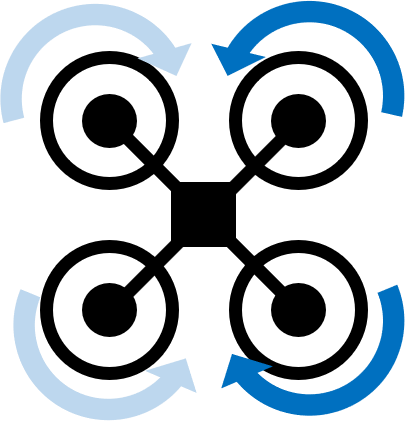
\includegraphics[scale=0.4]{img/drone_x_roll}
		\caption{Roll left}
		\label{fig:x-roll}
	\end{subfigure}
	~
	\begin{subfigure}[b]{0.3\textwidth}
		\centering
		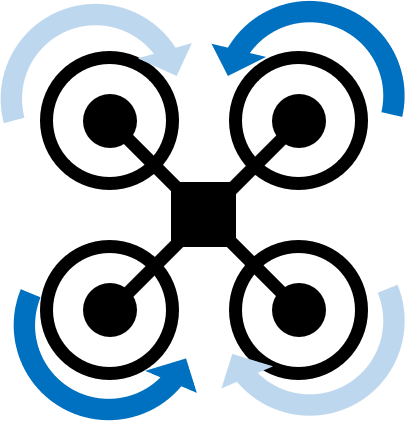
\includegraphics[scale=0.4]{img/drone_x_yaw}
		\caption{Yaw left}
		\label{fig:x-yaw}
	\end{subfigure}
	
	\caption{Using differential thrust to obtain 6-DOF movement. }
	\label{fig:rpas_6dof}
\end{figure}

A multirotor has several common configurations such as tricopter, quadcopter, hexacopter as depicted in Figure~\ref{fig:rpas-config}. Because each frame has different layouts of motors, the forces acting on the drone is inherently different and thus provides advantages and disadvantages of their own.

We use a quadcopter X4 configuration (4 motors and propellers in the shape of a letter X) for our multirotor as it is easy to control and provides abundant control system robustness. Such configuration is also the most popular amongst the UAS industry because it is balances redundancy and robustness with capacity and performance.

As seen in Figure \ref{fig:quadcopter-x-t}. Two of the motors spin clockwise and the other two spin counter-clockwise --- effectively canceling each other's unintended torque applied to the multirotor. Applying the same power into each motor allows the MRPAS to hover in place. We can perform 6 degree-of-freedom (DOF) movements by applying a combination of differential thrusts to each motor (Figure \ref{fig:rpas_6dof}). An X4 configuration is inherently stable.

A dual-blade helicopter, for example, requires fewest number of motors. But like a single-blade helicopter, the system in control theory sense, is naturally unstable and requires difficulty to stabilize the system. A tricopter has odd number of motors which also shares similar characteristics with a helicopter where the system requires an additional tail motor to compensate for the uneven torque. 

Configurations using more than 4 motors such as a hexacopter or an octocopter are very expensive for the amount of parts they require. Drones of these configuration classes are very stable with failure redundancy. However, these drones are typically much larger (0.6m to 1.5m wide) and much heavier (up to 25 kg). As a result, they are typically used in industrial, filming, and agriculture applications with a typical unit cost of at least several thousand dollars. These configurations are not suitable for our applications.

\paragraph{Airframe}

\begin{figure}[h]
	\centering
	\begin{subfigure}[b]{0.33\textwidth}
		\centering
		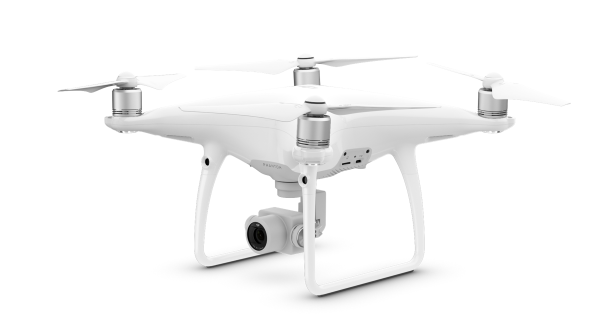
\includegraphics[width=\textwidth]{img/djiphantom4}
		\caption{DJI Phantom 4 (350 mm)}
		\label{fig:djiphantom}
	\end{subfigure}
	~
	\begin{subfigure}[b]{0.33\textwidth}
		\centering
		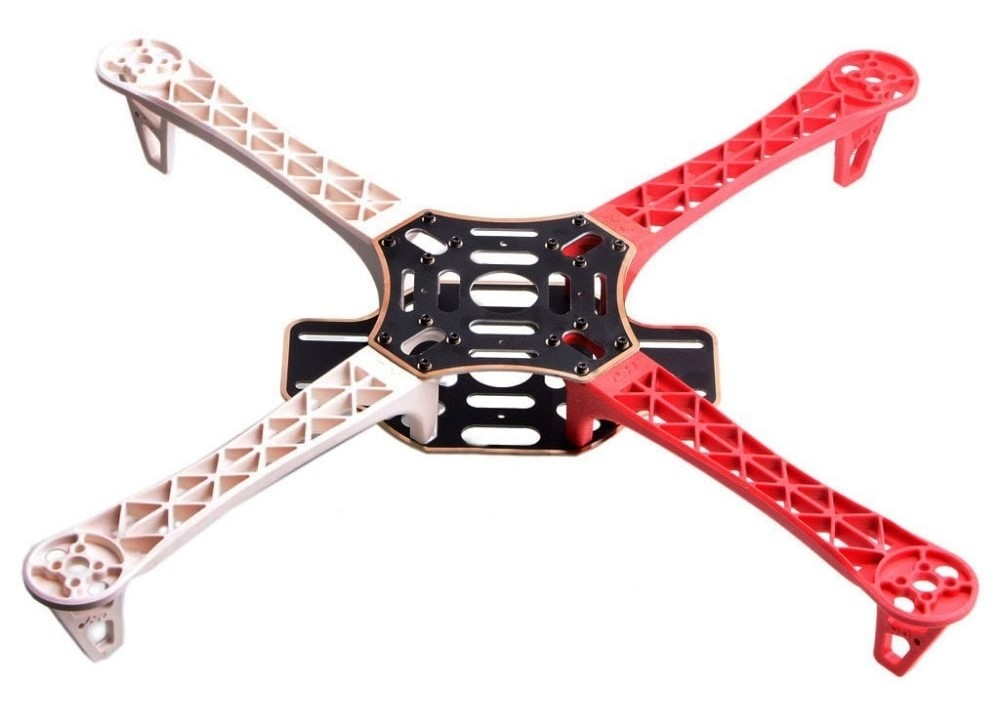
\includegraphics[width=\textwidth]{img/f450frame}
		\caption{Generic DIY frame kit (450 mm)}
	\end{subfigure}
	~
	\begin{subfigure}[b]{0.33\textwidth}
		\centering
		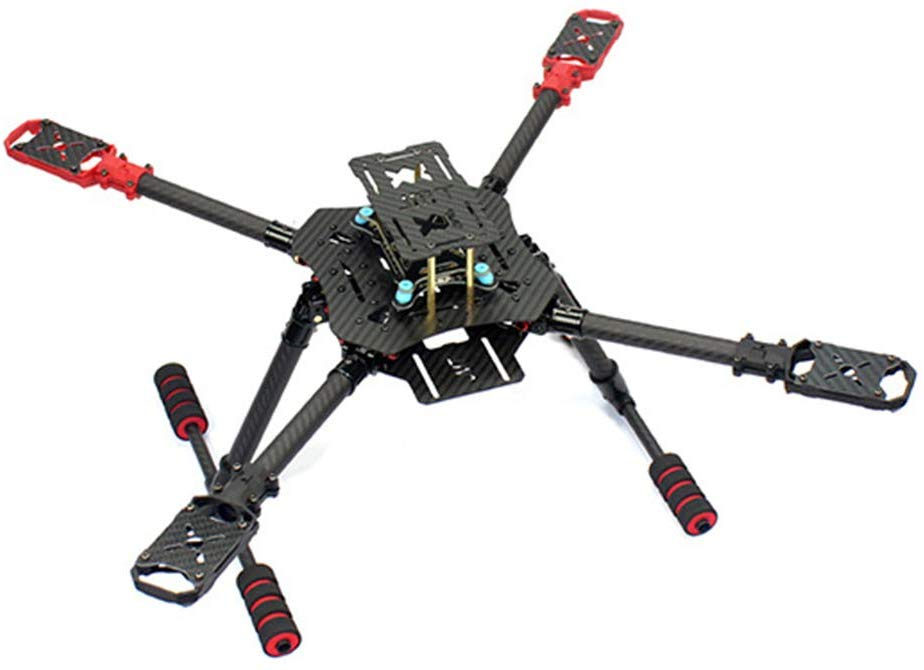
\includegraphics[width=\textwidth]{img/jmt560}
		\caption{JMT X4 Carbon Fiber Frame (560 mm)}
		\label{fig:jmtx4}
	\end{subfigure}
	~
	\begin{subfigure}[b]{0.33\textwidth}
		\centering
		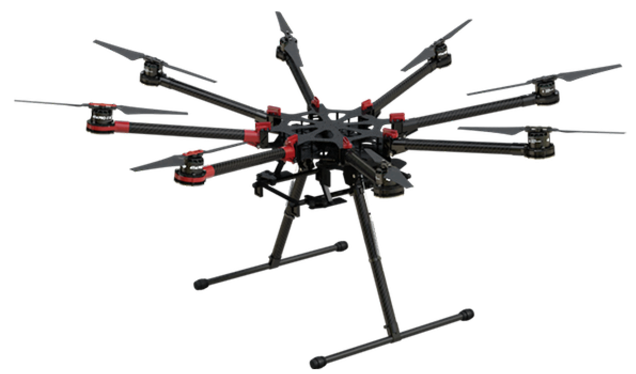
\includegraphics[width=\textwidth]{img/djis1000}
		\caption{DJI Spreadwings S1000 (1000 mm)}
		\label{fig:djis1000}
	\end{subfigure}
	
	\caption{Air Frame Options with Various Size Tiers }
\end{figure}

Multirotor airframe sizes are commonly designated by their \textit{motor-to-motor-diagonal-span} (MMDS), which measures the distance between the pair of motors which are the furthest apart. 

We adopt a X4 560 mm MMDS carbon fibre frame from JMT, as shown in Figure~\ref{fig:jmtx4}. The frame is carbon fibre to enhance structural rigidity while keeping the system relatively lightweight. The frame features foldable arms and landing gears for portability, but we consider replacing the hinges with static parts to reduce  weight and achieve a longer flight time. The X4 560 mm frame is also wide enough to support propellers up to 14 inches in diameter. The carbon fibre material is light, strong, and rigid. Although this means that the items mounted on the frame would suffer from lack of dampening of vibrations, we implement compensating dampers for sensors separately.

The 350 mm frames are also popular amongst consumer products such as the DJI Phantom series\cite{dji-phantom-3-specs} as seen in Figure~\ref{fig:djiphantom}. A frame size of 350 mm would constrain our ability to mount larger hardware --- posing a significant risk to integrating computing platform hardware. Additionally, the 350 mm size also limits the propeller maximum size. The largest quadcopter configurations have an MMDS of 1000 mm to allow for extremely large payload capacities such as the one shown in Figure~\ref{fig:djis1000}. However, these are more commonly used for industrial or military applications.

\paragraph{Customized Add-ons}
% TODO: add CAD parts

\subsubsection{Propulsion}

The propulsion system covers the majority of the multirotor parts list and determines the flight performance of the multirotor. We refer to this subsystem as the ``Drive".

\paragraph{Motor Type}

\underline{\textit{Brushed or brushless?}}
Multirotors are electrically powered by a battery --- a DC source. Two common types of DC motors are  brushed motors and brushless DC (BLDC) motors. Brushed motors commutate mechanically using brushes whereas brushless motors commutate electrically using electronic controllers that switches phases in the stator coils.

We use  BLDC motors for their extended usable lifespan and efficiency. Brushed motors are not appropriate for our applications for its excessive noise, friction, spark, and heat.

\underline{\textit{Inrunner or outrunners?}}

BLDC motors further consists of two variants: \textit{inrunner} and \textit{outrunner}. 

We choose outrunner BLDC motors for its higher torque output at lower speed  (i.e. outrunner motors have low KV constants; see Appendix~\ref{appendix:droneengine} for KV relationships). The lower speed of the rotor is beneficial for two reasons. One, a motor running at a lower speed is more efficient and produces less high frequency vibrations. Two, the attached propeller can be much larger and cut through the air at a lower speed, since drag forces acting on the blades are proportional to the velocity squared. Outrunner motors do require spin-up time as the rotor is more massive and has more inertia, but this compromise is acceptable as the main operating mode of the multirotor is hovering, which requires little agility. 

The alternatives are inrunner motors. Inrunner motors have the rotor on the inside and outrunner motors have the rotor on the outside. Inrunner rotors are lighter and spin faster with a lower torque which means additional gearboxes are required to extract useful torque\cite{invsoutrunner}.

\paragraph{Motor Size and Speed}\label{section:motor-speed}

Commercial outrunner BLDC motors generally have the following design parameters: stator size, KV/KT constants, voltage, maximum rated power, and weight. Please refer to Appendix~\ref{appendix:droneengine} for the relationship between the aforementioned design parameters. 

We choose 700 KV motors with stator size 3508.  According to drone hobbist online sources (https://quadquestions.com/blog/2017/02/22/choose-right-size-motors-drone/, https://oscarliang.com/quadcopter-motor-propeller/), the ideal KV motors to maximize performance for frame sizes larger than 450 mm should be 1200 KV or less. The argument of choosing a lower KV motor follows the point made above to balance torque output and energy loss due to air friction.

Our decision process consists of screening and ranking the best motors through applying priorities as follows:

\begin{enumerate}
    \item Voltage: We chose a motor that operates between 12.0 V and 20.0 V, which is enough for heavy operations.
    \item KV constant: Since the motors' RPM-per-volt ratio (KV constant) is inversely proportional of torque-per-current ratio (KT constant), manufacturers typically only focus on the KV constant. We chose motors that have KV constants between 500 KV and 1000 KV. These constants are considered low-speed and high-torque, and are typically used for large drones and endurance flights. We also chose this range such that the propellers can spin slower and more efficiently, extending the maximum flight time.
    \item Rotor size: As mentioned in the previous section regarding inrunners vs. outrunners, larger rotors imply a lower KV and higher KT. As a result, we chose motors within the 500 KV to 1000 KV range. Markets show that sizes denoted 3508 to 2212 are adequate for this purpose.
    \item Maximum rated power: KV and KT constants are a simplified model for motor characteristics. The maximum power output is derived when considering realistic non-idealities such as heat, motor resistance, and mechanical limits. Typically 500 KV to 1000 KV motors have a rating between 150 W to 400 W, depending on the brand. We optimize for the most performant option allotted by our budget.
    \item Weight: Given that the weight of motors have little variance, we prioritize this parameter the least.
\end{enumerate}

\paragraph{Electronic Speed Controllers}

Electronic speed controllers (ESC) control the voltage, current, and phase supplied to a BLDC motor. As BLDC motors function by rotating magnetic fields using electric commutation, the ESCs must precisely control the timing and phase of the input. All ESCs function similarly and the design parameters are size/weight, power rating, power efficiency, and cost. We use HobbyWing XRtoor 40.0 A  ESCs (https://imgaz.staticbg.com/images/upload/2014/12/Hobbywing\%20xRotor\%20Manual.pdf).

\paragraph{Propellers}

Common RPAS propellers are constructed using either plastic or carbon fibre. For the final deliverable we utilize carbon fiber propellers to maximize efficiency, flight time, and longevity for our client. 

According to Oscar Liang (https://www.dronethusiast.com/carbon-fiber-props-vs-plastic/),  carbon fibre propellers are tough and rigid and produces efficient and low-noise flight performance.  While plastic propellers are cheap, abundant, and relatively flexible, the manufacture of plastic propellers is not as precise, which leads to aerodynamic inefficiencies. Plastic propellers often require balancing, where one applies tape to the blades such that the weight on each blade is balanced. 

We choose propellers with size 1250. Where 12 denotes 12 inches in diameter, and 50 denotes 5.0 inches in propeller pitch. To obtain maximum thrust and minimize speed (low speed is more desirable, as mentioned in Section \ref{section:motor-speed}), we strike a balance if we choose 11 to 13 inch propellers to be fitted onto the multirotor.

\begin{figure}[h]
    \centering
    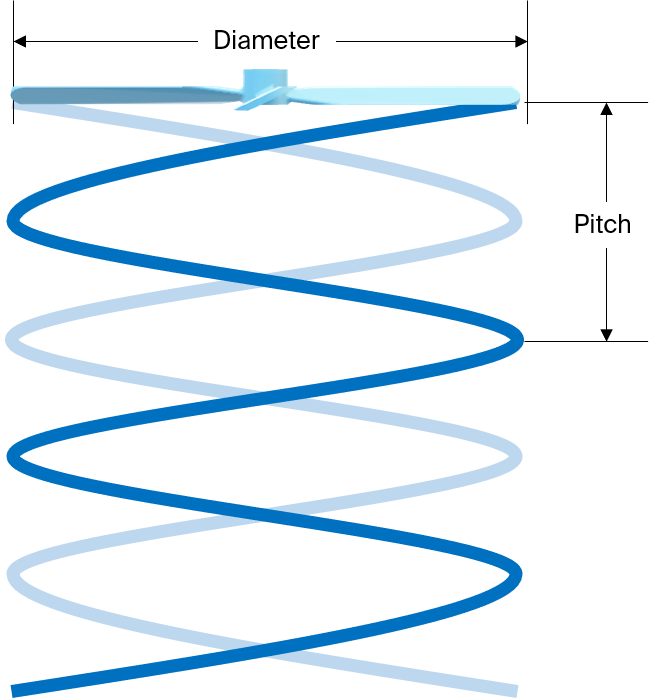
\includegraphics[scale=0.5]{img/proppitch}
    \caption{Propellor Diameter and Pitch Parameters}
    \label{fig:propeller}
\end{figure}

\begin{figure}[h]
    \centering
    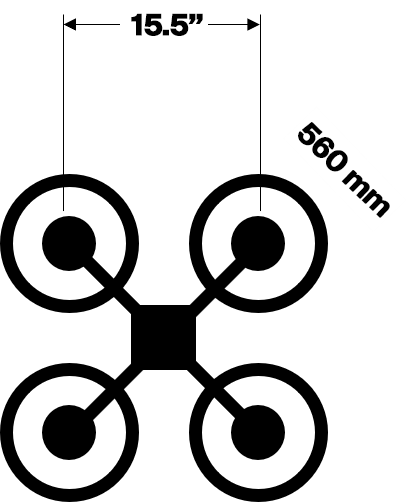
\includegraphics[scale=0.5]{img/framepropsize}
    \caption{Maximum Propeller Sizes}
    \label{fig:framepropsize}
\end{figure}

As mentioned in Section \ref{section:drone-mech} the frame size is 560 mm (22 inches), which means that the motor to motor adjacent span is about 15.5 inches (by dividing by $\sqrt{2}$). It is safe to provide several inches of clearance between propellers, therefore the  compatible size of propellers are between 11 to 14 inches.

Mentioned in Section \ref{section:motor-speed}, we chose low-speed motors for their efficiency. Additionally recall that, given the same power, a slow-speed motor provides inversely proportional torque, so we chose propellers with relatively high pitch (between 3 to 5 inches) to take advantage of the high-torque output in maximizing thrust output.

\subsubsection{Battery and Electrical Systems}
\paragraph{Battery Type}
\paragraph{Battery Capacity}
\paragraph{Power Distribution}

\subsubsection{Flight Computer and Sensors}
\paragraph{Flight Computer Unit}
\paragraph{Sensors}
\paragraph{Flight Modes}
\paragraph{FCU Software}

\subsubsection{Communication and Control}
\paragraph{Transmitter}
\paragraph{Receiver}